\documentclass[10pt]{revtex4-2}
\usepackage{braket,amsmath,amssymb,graphicx,float,hyperref,paralist}
\numberwithin{equation}{section}
\allowdisplaybreaks
\usepackage[utf8]{inputenc}
\usepackage[T1]{fontenc}
\usepackage{ebgaramond}
\begin{document}
\title{Multi-channel Kondo model URG}
\author{Abhirup Mukherjee}
\date{\today}
\maketitle
\section{Derivation of URG equations for the multi-channel Kondo model}

\subsection{Introduction}
The multi-channel Kondo model is described by the Hamiltonian
\begin{equation}\begin{aligned}
	H = \sum_{k,\alpha,\gamma}\epsilon_{k}^\gamma \hat n^\gamma_{k\alpha} + J\sum_{kk^\prime,\gamma} \vec{S_d}\cdot\vec{s}_{\alpha\alpha^\prime}{c^\gamma_{k\alpha}}^\dagger c^\gamma_{k^\prime\alpha^\prime}~.
\end{aligned}\end{equation}
It is mostly identical to the single-channel Kondo model: \(k,k^\prime\) sum over the momentum states, \(\alpha,\alpha^\prime\) sum over the spin indices and \(\gamma\) sums over the various channels. \(\vec S_d, \vec s\) are the impurity and conduction bath spin vectors. The renormalization at step \(j\) is given by
\begin{equation}\begin{aligned}
	\Delta H_j = \left(c^\dagger T \frac{1}{\hat \omega - H_D}T^\dagger c + T^\dagger c \frac{1}{\hat \omega - H_D}c^\dagger T\right), && c^\dagger T = J \sum_{k < \Lambda_j, \alpha}\vec{S_d}\cdot\vec{s}_{\beta \alpha}c^\dagger_{q\beta}c_{k\alpha}, &H_D = \epsilon_q \tau_{q\beta} + J S_d^z s_q^z
\end{aligned}\end{equation}
Usually we treat the \(\hat \omega\) as number(s) and study the renormalization in the couplings as functions of the quantum fluctuation scales. Each value of the fluctuation scale defines an eigendirection of \(\hat \omega\). We have then essentially traded off the complexity in the non-commutation of the diagonal and off-diagonal terms for all the directions in the manifold of \(\hat \omega\).

Here we will do something different. We will redefine the \(\hat \omega\) by pulling out the off-diagonal term from it: \(\hat \omega \to \hat \omega - H_X\), and then study the renormalization at various orders by expanding the denominator in powers of \(H_X\). Such a redefinition essentially amounts to a rotation of the eigendirections of \(\hat \omega\). This is done in order to extract some information out of \(\hat \omega\), specifically the dependence of the RG equations on the channel number \(K = \sum_\gamma\). This dependence is in principle present even if we do not do such a redefinition and expansion, in the various directions and values of \(\omega\), because those values encode the non-perturbative information regarding scattering at all loops. However, it is difficult to read off this information directly. This step of redefinition followed by expansion is being done with the sole aim of exposing such information. 

The expansion we are talking about is
\begin{equation}\begin{aligned}
	\eta = \frac{1}{\hat \omega - H_D}T^\dagger c = \frac{1}{\omega^\prime - H_D - H_X}T^\dagger c \simeq \frac{1}{\omega^\prime - H_D}T^\dagger c + \frac{1}{\omega^\prime - H_D}H_X \frac{1}{\omega^\prime - H_D} T^\dagger c
\end{aligned}\end{equation}
where \(H_X = J \sum_{k,k^\prime < \Lambda_j, \alpha,\alpha^\prime}\vec{S_d}\cdot\vec{s}_{\alpha \alpha^\prime}c^\dagger_{k\alpha}c_{k^\prime\alpha^\prime}\) is scattering between the entangled electrons.
With this change, the second and third order renormalizations will take the form
\begin{equation}\begin{aligned}
	\Delta H^{(2)}_j = c^\dagger T \frac{1}{\omega^\prime - H_D}T^\dagger c + T^\dagger c \frac{1}{\omega - H_D}c^\dagger T
\end{aligned}\end{equation}
\begin{equation}\begin{aligned}
	\Delta H^{(3)}_j = c^\dagger T \frac{1}{\omega^\prime - H_D} H_X \frac{1}{\omega^\prime - H_D} T^\dagger c + T^\dagger c \frac{1}{\omega - H_D} H_X \frac{1}{\omega - H_D} c^\dagger T
\end{aligned}\end{equation}
We will use the identity
\begin{equation}\begin{aligned}
	\label{identity_SSS}
	S_d^a S_d^z S_d^b = \left(\frac{1}{4}\delta^{az} + \frac{i}{2}\sum_c \epsilon^{azc}S_d^c\right)S_d^b = \left(\frac{1}{4}\delta^{az}S_d^b + \frac{i}{8} \epsilon^{azb}  - \frac{1}{4}\sum_{c_1,c} \epsilon^{azc_1} \epsilon^{c_1 b c} S_d^c\right) = \frac{1}{4}\left(\delta^{az}S_d^b - \delta^{ab}S_d^z + \delta^{bz}S_d^a\right)
\end{aligned}\end{equation}

\subsection{Leading order renormalization}
\begin{equation}\begin{aligned}
	\Delta H^{(2)}_j = \underbrace{c^\dagger T \frac{1}{\omega^\prime - H_D}T^\dagger c}_\text{first term}~+~\underbrace{T^\dagger c \frac{1}{\omega - H_D}c^\dagger T}_\text{second term}
\end{aligned}\end{equation}
This renormalization is identical to that in the single channel. There is no additional physics due to the presence of multiple channels at this order. It is shown in appendix \ref{1KondoURG}.

\subsection{Next-to-leading order renormalization}
\begin{equation}\begin{aligned}
	\Delta H^{(3)}_j = \underbrace{c^\dagger T \frac{1}{\omega^\prime - H_D} H_X \frac{1}{\omega^\prime - H_D} T^\dagger c}_\text{first term} ~+~ \underbrace{T^\dagger c \frac{1}{\omega - H_D} H_X \frac{1}{\omega - H_D} c^\dagger T}_\text{second term}
\end{aligned}\end{equation}
A general term of this summation has three sets of spin operators coming from \(c^\dagger T, H_X\) and \(T^\dagger c\). If we had expressed the spin operators in terms of \(S^z, S^\pm\), most of the terms would have atleast one \(S^+\) or \(S^-\), and by the same argument as in the single-channel case, the denominator will have anti-parallel spins and the Ising term will be negative, leading to the form: \(\omega - D/2 - \epsilon_k/2 + J/4\). \(\epsilon_k\) is the energy of the other electron that will be summed over. The only term that does not have even one \(S^\pm\) is the one with three \(S^z\). We can show that this term will also have the same denominator. An instance of this term (in shorthand) is
\begin{equation}\begin{aligned}
	S_d^z c^\dagger_{q \uparrow} \frac{1}{\omega - D/2 -\epsilon_k/2 + J/2 S_d^z} S_d^z \frac{1}{\omega - D/2 -\epsilon_k/2 + J/2 S_d^z} S_d^z c_{q \uparrow}\\
\end{aligned}\end{equation}
This can be split into up and down configurations of the impurity spin using the decomposition \(S_d^z = \frac{1}{2}\left(\frac{1}{2} + S_d^z\right) - \frac{1}{2}\left(\frac{1}{2} - S_d^z \right) \). These configurations will have different quantum fluctuation scales \(\omega, \omega^\prime\):
\begin{equation}\begin{aligned}
	\frac{1}{2}S_d^z c^\dagger_{q \uparrow}\left[\frac{\left(\frac{1}{2} + S_d^z\right)}{\left(\omega - D/2 -\epsilon_k/2 + J/4\right)^2} - \frac{\left(\frac{1}{2} - S_d^z\right)}{\left(\omega^\prime - D/2 -\epsilon_k/2 - J/4\right)^2}\right]S_d^z c_{q \uparrow}
\end{aligned}\end{equation}
If we now use poor man's scaling values to relate the two \(\omega\)s, we get \(\omega^\prime - \omega = J/2\). Substituting this will make both the denominators identical: \(\omega - D/2 -\epsilon_k/2 + J/4\). This means that the denominator for all non-zero terms that renormalize the Hamiltonian is \(\omega - D/2 - \epsilon_k/2 + J/4\).

\subsubsection{Calculation of first term}
\begin{equation}\begin{aligned}
	c^\dagger T \frac{1}{\omega^\prime - H_D} H_X \frac{1}{\omega^\prime - H_D} T^\dagger c = J^3\sum_{q, k, k_1,k_2,\atop{\beta, \alpha, \alpha_1,\alpha_2,\atop{l_1,l_2,a,b,c}}} \frac{c^\dagger_{q\beta,l_1} c_{k\alpha,l_1} S_d^a s^a_{\beta \alpha} S_d^b s^b_{\alpha_1 \alpha_2} c^\dagger_{k_1\alpha_1,l_2}c_{k_2 \alpha_2,l_2} c^\dagger_{k\alpha, l_1} c_{q\beta, l_1} S_d^c s^c_{\alpha \beta}}{\left(\omega - D/2 -\epsilon_k/2 + J/4\right)^2}
\end{aligned}\end{equation}
\(q\) sums over the momenta being decoupled. \(k, k_1,k_2\) sum over the momenta not being decoupled. \(\beta, \alpha, \alpha_1,\alpha_2\) sum over the spin indices. \(l_1,l_2\) sum over the channels. We will start simplifying this equation by summing over \(q\). \(c^\dagger_{q\beta}\) and \(c_{q\beta}\) can be easily combined to form \(\hat n_{q\beta}\), because they anti-commute with the other momenta. The sum gives \(\sum_q \hat n_{q\beta l_1} = n(D) \). This gives
\begin{equation}\begin{aligned}
	c^\dagger T \frac{1}{\omega^\prime - H_D} H_X \frac{1}{\omega^\prime - H_D} T^\dagger c = J^3 n(D)\sum_{k, k_1,k_2,\atop{\beta, \alpha, \alpha_1,\alpha_2,\atop{l_1,l_2,a,b,c}}} \frac{c_{k\alpha,l_1} S_d^a s^a_{\beta \alpha} S_d^b s^b_{\alpha_1 \alpha_2} c^\dagger_{k_1\alpha_1,l_2}c_{k_2 \alpha_2,l_2} c^\dagger_{k\alpha, l_1} S_d^c s^c_{\alpha \beta}}{\left(\omega - D/2 -\epsilon_k/2 + J/4\right)^2}
\end{aligned}\end{equation}
The operators \(c^\dagger_{k\alpha}\) and its conjugate can be brought together without any change of sign because there will be an even number of flips. The sum over \(k\) gives
\begin{equation}\begin{aligned}
	\sum_k \frac{1 - \hat n_{k\alpha l_1}}{\left(\omega - D/2 -\epsilon_k/2 + J/4\right)^2} =  \rho\int \frac{d\epsilon\left[1 - \hat n(\epsilon)_{\alpha l_1}\right] }{\left(\omega - D/2 -\epsilon/2 + J/4\right)^2} = \rho\int_0^{D-2\left( \omega + J/4 \right) } \frac{d\epsilon}{\left(\omega - D/2 -\epsilon/2 + J/4\right)^2}
\end{aligned}\end{equation}
The integration goes over positive energies only because of the \(1 - \hat n\) operator; the upper limit of the integration is chosen so as to make the denominator double, because this preserves the symmetry of the denominator and this is what happens in poor man's scaling. Performing the integration gives
\begin{equation}\begin{aligned}
	\sum_k \frac{1 - \hat n_{k\alpha l_1}}{\left(\omega - D/2 -\epsilon_k/2 + J/4\right)^2} = -\frac{1}{2}\frac{\rho}{\omega - D/2 + J/4}
\end{aligned}\end{equation}
The sum over the channel index \(l_1\) produces a factor of \(K\). \(K = \sum_{l_1}\) is the total number of conduction bath channels. The entire expression is now
\begin{equation}\begin{aligned}
	\label{first_term}
	c^\dagger T \frac{1}{\omega^\prime - H_D} H_X \frac{1}{\omega^\prime - H_D} T^\dagger c = -\frac{1}{2}\frac{J^3 n(D) \rho K}{\omega - D/2 + J/4}\sum_{\beta, \alpha, \alpha_1,\alpha_2,\atop{a,b,c}} S_d^a s^a_{\beta \alpha} S_d^b s^b_{\alpha_1 \alpha_2} S_d^c s^c_{\alpha \beta} \sum_{k_1,k_2,l_2} c^\dagger_{k_1\alpha_1,l_2}c_{k_2 \alpha_2,l_2}
\end{aligned}\end{equation}
We now need to simplify the spin products. The sum over \(\alpha,\beta\) can be carried out immediately: \(\sum_{\alpha,\beta} s^a_{\beta \alpha} s^c_{\alpha \beta} = \text{Trace}\left(s^a s^c\right) = \frac{1}{2}\delta^{ac}\). Substituting this gives
\begin{equation}\begin{aligned}
	c^\dagger T \frac{1}{\omega^\prime - H_D} H_X \frac{1}{\omega^\prime - H_D} T^\dagger c = -\frac{1}{2}\frac{J^3 n(D) \rho K}{\omega - D/2 + J/4}\frac{1}{2}\sum_{\alpha_1,\alpha_2,a,b} S_d^a S_d^b S_d^a \sum_{k_1,k_2,l_2} c^\dagger_{k_1\alpha_1,l_2}c_{k_2 \alpha_2,l_2}s^b_{\alpha_1 \alpha_2} 
\end{aligned}\end{equation}
The spin product can now be carried out:
\begin{equation}\begin{aligned}
	\sum_a S_d^a S_d^b S_d^a = \sum_a S_d^a\left[\frac{1}{4}\delta^{ab} + \frac{i}{2}\sum_c \epsilon^{bac}S_d^c\right] = \frac{1}{4}S_d^b - \frac{1}{4}\sum_{ace}\epsilon^{bac}\epsilon^{ace}S_d^e = \frac{1}{4}S_d^b - \frac{1}{4}S_d^b \sum_{ac}\epsilon^{bac}\epsilon^{acb} \\
	= -\frac{1}{4}S_d^b
\end{aligned}\end{equation}
The renormalization becomes
\begin{equation}\begin{aligned}
	\Delta H_1 = c^\dagger T \frac{1}{\omega^\prime - H_D} H_X \frac{1}{\omega^\prime - H_D} T^\dagger c = -\frac{1}{2}\frac{J^3 n(D) \rho K}{\omega - D/2 + J/4}\frac{1}{2}\left( -\frac{1}{4} \right) \sum_{k_1,k_2,\alpha_1,\alpha_2,b} S_d^b s^b_{\alpha_1 \alpha_2} c^\dagger_{k_1\alpha_1,l_2}c_{k_2 \alpha_2,l_2}\\
=\frac{1}{16}\frac{J^3 n(D) \rho K}{\omega - D/2 + J/4} \sum_{k_1,k_2,\alpha_1,\alpha_2} \vec{S_d}\cdot\vec{s}_{\alpha_1 \alpha_2} c^\dagger_{k_1\alpha_1,l_2}c_{k_2 \alpha_2,l_2}
\end{aligned}\end{equation}

\subsubsection{Calculation of second term}
Like the single-channel case, the renormalization coming from the hole excitations is exactly the Hermitian conjugate of that in the particle sector. And since the renormalization \(\Delta H_1\) is Hermitian, we have \(\Delta H_0 = \Delta H_1\)

\subsection{Total renormalization \(\Delta H^{(3)}\)}
The total renormalization is twice that in the particle sector.
\begin{equation}\begin{aligned}
	\Delta H^{(3)} = \frac{1}{8}\frac{J^3 n(D) \rho K}{\omega - D/2 + J/4} \sum_{k_1,k_2,\alpha_1,\alpha_2} \vec{S_d}\cdot\vec{s}_{\alpha_1 \alpha_2} c^\dagger_{k_1\alpha_1,l_2}c_{k_2 \alpha_2,l_2}
\end{aligned}\end{equation}
Combining with \(\Delta H^{(2)}\) and replacing \(n(D) = \rho |\delta D|\), we get
\begin{equation}\begin{aligned}
	\frac{\Delta J}{|\Delta D|} = -\frac{J^2 \rho}{\omega - D/2 + J/4} + \frac{1}{8}\frac{J^3 \rho^2 K}{\omega - D/2 + J/4} = -\frac{J^2 \rho}{\omega - D/2 + J/4}\left[1 - \frac{1}{8}J\rho K\right] 
\end{aligned}\end{equation}
We choose \(\omega = -D/2\) to get a clearer idea of what the equations say. 
\begin{equation}\begin{aligned}
	\label{mchannel}
	\frac{\Delta J}{|\Delta D|} = \frac{J^2 \rho}{D - J/4}\left[1 - \frac{1}{8}J\rho K\right] 
\end{aligned}\end{equation}
Quantities with zero in the subscript will denote their values in the bare Hamiltonian. Using \(\delta D = -|\delta D|\), we can write the continuum form of the equation:
\begin{equation}\begin{aligned}
	\frac{\:\mathrm{d}J}{\:\mathrm{d}D} = \frac{J^2 \rho}{D - J/4}\left(\frac{1}{8}J\rho K - 1\right)
\end{aligned}\end{equation}

For \(D \gg J\), we can ignore the \(J\) in the denominator, and the equation reduces to the one-loop poor man's scaling form
\begin{equation}\begin{aligned}
	\label{pms_mchannel}
	\frac{\:\mathrm{d}J}{\:\mathrm{d}D} \simeq  \frac{J^2 \rho}{D}\left(\frac{1}{8}J\rho K - 1\right)
\end{aligned}\end{equation}
This equation has a stable fixed point at \(J^* = \frac{8}{\rho K}\).

\begin{figure}[!htb]
	\centering
	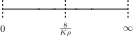
\includegraphics[width=0.4\textwidth]{rg_flow_pms.pdf}
	\caption{Attractive finite \(J\) fixed point of poor man scaling RG equation}
\end{figure}
For \(D\) not so large, the denominator also comes into play, and eq.\ref{mchannel} holds. We get the possibility of two fixed points - one from the numerator and the other from the numerator.
\begin{figure}[!htb]
	\centering
	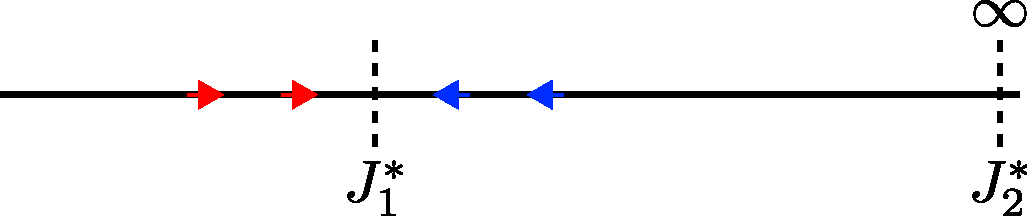
\includegraphics[width=0.7\textwidth]{./rg_flow.pdf}
	\caption{}
	\label{rg_flow_general}
\end{figure}

The numerator and denominator fixed points, \(J_1^*\) and \(J_2^*\) respectively, are given by
\begin{equation}\begin{aligned}
	J_1^* = \frac{8}{K \rho}, && D^* = \frac{J_2^*}{4}
\end{aligned}\end{equation}
For a given \(K\), the position of \(J_1^*\) will be governed by \(\rho\). In general, for each bare bandwidth \(D_0\), there exists a minimal \(\rho\), $\rho_\text{min}(D_0)$, above which the the lower fixed point is the one from the numerator. That is, for \(\rho > \rho_\text{min}\), if we start scaling from small \(J_0\), it grows until it hits \(J_1^*\) which acts as the attractive fixed point, and \(J_2^*\) lies at a higher value and acts as the repulsive fixed point. For \(\rho < \rho_\text{min}\), \(J\) will grow and hit \(J_2^*\) instead, and \(J_1^* > J_2^*\) now becomes the repulsive fixed point.
\begin{equation}\begin{aligned}
	\rho_\text{min} = \text{minimum }\left\{\rho, \text{ such that } \frac{8}{K \rho} < 4 D^*(\rho)\right\}
\end{aligned}\end{equation}
This behaviour is shown schematically in fig.~\ref{rg_flow_general}. 
In fig.~\ref{rhomin_vs_D}, we plot \(\rho_\text{min}\) against the bare bandwidth. For large \(D_0\), it essentially shrinks to zero, and the numerator becomes the first fixed point for essentially all \(\rho\).
\begin{figure}[!htb]
	\centering
	\includegraphics[width=0.7\textwidth]{./rhomin_D.pdf}
	\caption{Red curve shows variation of \(\rho_\text{min}\) against \(D_0\). It vanishes at large \(D_0\). Blue curve shows variation of the ratio \(J_1^* / D_0\) with \(D_0\). That shrinks as well, showing that the fixed point \(J_1^*\) remains finite in the thermodynamic limit, and the distance between \(J_1^*\) and \(J_2^*\) keeps growing.}
	\label{rhomin_vs_D}
\end{figure}

If we assume we are at a sufficiently large \(D_0\) and \(\rho > \rho_\text{min}\), the lower fixed point is \(J_1^*\). As shown in fig.~\ref{rhomin_vs_D}, we have \(J_1^* \ll D_0\). If we start with \(J_0\) in the neighborhood of \(J_1^*\), we can use \(J_1^* \ll D_0\) to ignore \(J\) in the denominator and the RG equation reduces to the poor man's scaling form eq.~\ref{pms_mchannel}. The denominator fixed point has effectively moved off to infinity. That this is true can also be argued from the single-channel Kondo model URG results. There, we saw that when the bandwidth is scaled to larger values, the strong-coupling fixed point was stable at successively larger values of \(J^*\). Since the denominator fixed point is identical in structure in both problems, its reasonable that the same thing will happen here.

\section{Derivation of low energy effective Hamiltonian \((k-\text{space})\)}
Fixed point Hamiltonian is
\begin{equation}\begin{aligned}
	H^* = H_0 + J^*\sum_{l} \vec{S_d}\cdot\vec{s_\text{tot}}
\end{aligned}\end{equation}
where \(H_0 = \sum_{k,l,\sigma}\epsilon_{k,l}\hat n_{k\sigma,l}\) and \(\vec s_\text{tot} = \sum_l \vec s_l = \sum_{kk^\prime\alpha\alpha^\prime,l} \vec \sigma_{\alpha\alpha^\prime}c^\dagger_{k\alpha,l}c_{k^\prime\alpha^\prime,l}\). \(l\) sums over the channels. Henceforth we will drop the \(*\). Obtaining the effective Hamiltonian involves obtaining the low energy excitations on top of this fixed point Hamiltonian. The large-energy excitations are ones that involve spin flips. This guides the separation of the Hamiltonian into a diagonal and an off-diagonal piece:
\begin{equation}\begin{aligned}
	H = H_d + V = \underbrace{H_0 + J S_d^z s_\text{tot}^z}_{H_d} + \underbrace{\frac{J}{2}S_d^+ s_\text{tot}^- + \text{h.c.}}_V
\end{aligned}\end{equation}
The effective Hamiltonian that has the states \(\ket{S_d^z, s_\text{tot}, s_\text{tot}^z}\) as eigenstates are
\begin{equation}\begin{aligned}
	H_\text{eff} = H_d + V \frac{1}{E_\text{gs} - H_d}V = \sum_{k,l,\sigma}\epsilon_{k,l}\hat n_{k\sigma,l} + J S_d^z s_\text{tot}^z + \frac{J}{2}S_d^+ s_\text{tot}^- \frac{1}{E_\text{gs} - J S_d^z s_\text{tot}^z - H_0}\frac{J}{2}S_d^- s_\text{tot}^+\\
	+\frac{J}{2}S_d^- s_\text{tot}^+ \frac{1}{E_\text{gs} - J S_d^z s_\text{tot}^z - H_0}\frac{J}{2}S_d^+ s_\text{tot}^-
\end{aligned}\end{equation}
We can easily simplify the \(S_d^z\) in the denominator, because \(S_d^\pm \frac{1}{A + B S_d^z} = S_d^\pm \frac{1}{A \mp \frac{1}{2}B}\).
\begin{equation}\begin{aligned}
	H_\text{eff} = \sum_{k,l,\sigma}\epsilon_{k,l}\hat n_{k\sigma,l} + J S_d^z s_\text{tot}^z + \frac{J^2}{4} s_\text{tot}^- \frac{\frac{1}{2} + S_d^z}{E_\text{gs} + \frac{J}{2} s_\text{tot}^z - H_0} s_\text{tot}^+ + \frac{J^2}{4} s_\text{tot}^+ \frac{\frac{1}{2} - S_d^z}{E_\text{gs} - \frac{J}{2} s_\text{tot}^z - H_0} s_\text{tot}^-
\end{aligned}\end{equation}
Since \(H_0\) does not commute with the spin operators, we will need to expand the denominator to make sense of this Hamiltonian.
\begin{equation}\begin{aligned}
	 s_\text{tot}^- \frac{1}{E_\text{gs} + \frac{J}{2} s_\text{tot}^z - H_0} s_\text{tot}^+ =  s_\text{tot}^- \frac{1}{E_\text{gs} + \frac{J}{2} s_\text{tot}^z}\left[1 + \frac{1}{E_\text{gs} + \frac{J}{2} s_\text{tot}^z}H_0 + \frac{1}{E_\text{gs} + \frac{J}{2} s_\text{tot}^z}H_0\frac{1}{E_\text{gs} + \frac{J}{2} s_\text{tot}^z}H_0\right] s_\text{tot}^+\\
	 s_\text{tot}^+ \frac{1}{E_\text{gs} - \frac{J}{2} s_\text{tot}^z - H_0} s_\text{tot}^- =  s_\text{tot}^+ \frac{1}{E_\text{gs} - \frac{J}{2} s_\text{tot}^z}\left[1 + \frac{1}{E_\text{gs} - \frac{J}{2} s_\text{tot}^z}H_0 + \frac{1}{E_\text{gs} - \frac{J}{2} s_\text{tot}^z}H_0\frac{1}{E_\text{gs} - \frac{J}{2} s_\text{tot}^z}H_0\right] s_\text{tot}^-
\end{aligned}\end{equation}
This is an expansion in \(H_0^n/J^{n+1}, n=0,1,2,\ldots\). The \(n=0\) terms give
\begin{equation}\begin{aligned}
	s_\text{tot}^- \frac{1}{E_\text{gs} + \frac{J}{2} s_\text{tot}^z}s_\text{tot}^+ = s_\text{tot}^- s_\text{tot}^+ \frac{1}{E_\text{gs} + \frac{J}{2} \left(s_\text{tot}^z + 1\right)} %= \left[s_\text{tot}\left( s_\text{tot}+1 \right)  - s_\text{tot}^z\left( s_\text{tot}^z + 1 \right) \right] \frac{1}{E_\text{gs} + \frac{J}{2} \left(s_\text{tot}^z + 1\right)}\\ 
	\\
	s_\text{tot}^+ \frac{1}{E_\text{gs} - \frac{J}{2} s_\text{tot}^z}s_\text{tot}^- = s_\text{tot}^+ s_\text{tot}^- \frac{1}{E_\text{gs} - \frac{J}{2} \left(s_\text{tot}^z - 1\right)}% = \left[s_\text{tot}\left( s_\text{tot}+1 \right)  - s_\text{tot}^z\left( s_\text{tot}^z - 1 \right) \right] \frac{1}{E_\text{gs} - \frac{J}{2} \left(s_\text{tot}^z - 1\right)}
\end{aligned}\end{equation}

One of the \(n=1\) terms gives
\begin{equation}\begin{aligned}
	s_\text{tot}^- \frac{1}{E_\text{gs} + \frac{J}{2} s_\text{tot}^z}\frac{1}{E_\text{gs} + \frac{J}{2} s_\text{tot}^z}H_0 s_\text{tot}^+ =  \left(\frac{1}{E_\text{gs} + \frac{J}{2} \left(s_\text{tot}^z + 1\right)}\right)^2 s_\text{tot}^- H_0 s_\text{tot}^+ 
\end{aligned}\end{equation}
Next we calculate the commutator:
\begin{equation}\begin{aligned}
	\left[s_\text{tot}^+, H_0\right] = X^\dagger_{1,\text{tot}} = \sum_l X_{1,l}^\dagger = \sum_{kk^\prime,l}\left(\epsilon_k - \epsilon_{k^\prime}\right) c^\dagger_{k^\prime \uparrow} c_{k \downarrow}
\end{aligned}\end{equation}
where \(X_{n,l} \equiv \sum_{k,k^\prime}\left(\epsilon_k - \epsilon_{k^\prime}\right)^n c^\dagger_{k \downarrow}c_{k^\prime \uparrow} \).
Substituting this commutator gives
\begin{equation}\begin{aligned}
	s_\text{tot}^- \frac{1}{E_\text{gs} + \frac{J}{2} s_\text{tot}^z}\frac{1}{E_\text{gs} + \frac{J}{2} s_\text{tot}^z}H_0 s_\text{tot}^+ =  \left(\frac{1}{E_\text{gs} + \frac{J}{2} \left(s_\text{tot}^z + 1\right)}\right)^2 \left(s_\text{tot}^- s_\text{tot}^+ H_0 - s_\text{tot}^- X^\dagger_{1,\text{tot}}\right)
\end{aligned}\end{equation}
The other \(n=1\) term gives
\begin{equation}\begin{aligned}
	s_\text{tot}^+ \frac{1}{E_\text{gs} - \frac{J}{2} s_\text{tot}^z}\frac{1}{E_\text{gs} - \frac{J}{2} s_\text{tot}^z}H_0 s_\text{tot}^- =  \left(\frac{1}{E_\text{gs} - \frac{J}{2} \left(s_\text{tot}^z - 1\right)}\right)^2 \left(s_\text{tot}^+ s_\text{tot}^- H_0 + s_\text{tot}^+ X_{1,\text{tot}}\right)
\end{aligned}\end{equation}
One of the \(n=2\) terms gives
\begin{equation}\begin{aligned}
	&s_\text{tot}^- \frac{1}{E_\text{gs} + \frac{J}{2} s_\text{tot}^z}\frac{1}{E_\text{gs} + \frac{J}{2} s_\text{tot}^z}H_0 \frac{1}{E_\text{gs} + \frac{J}{2} s_\text{tot}^z}H_0 s_\text{tot}^+\\
	&= \left(\frac{1}{E_\text{gs} + \frac{J}{2} \left(s_\text{tot}^z + 1\right)}\right)^2 s_\text{tot}^- H_0 \frac{1}{E_\text{gs} + \frac{J}{2} s_\text{tot}^z}H_0 s_\text{tot}^+ \\
	&= \left(\frac{1}{E_\text{gs} + \frac{J}{2} \left(s_\text{tot}^z + 1\right)}\right)^2 s_\text{tot}^- H_0 \frac{1}{E_\text{gs} + \frac{J}{2} s_\text{tot}^z}\left(s_\text{tot}^+ H_0 - X^\dagger_\text{1,tot}\right) \\
	&= \left(\frac{1}{E_\text{gs} + \frac{J}{2} \left(s_\text{tot}^z + 1\right)}\right)^2 \left[s_\text{tot}^- H_0 s_\text{tot}^+\frac{1}{E_\text{gs} + \frac{J}{2} \left(s_\text{tot}^z+1\right)} H_0 - s_\text{tot}^- H_0\frac{1}{E_\text{gs} + \frac{J}{2}s_\text{tot}^z}X^\dagger_\text{1,tot}\right] \\
	&= \left(\frac{1}{E_\text{gs} + \frac{J}{2} \left(s_\text{tot}^z + 1\right)}\right)^2 \left[s_\text{tot}^- \left(s_\text{tot}^+H_0 - X^\dagger_{1,\text{tot}}\right)\frac{1}{E_\text{gs} + \frac{J}{2} \left(s_\text{tot}^z+1\right)} H_0 - s_\text{tot}^- H_0\frac{1}{E_\text{gs} + \frac{J}{2}s_\text{tot}^z}X^\dagger_\text{1,tot}\right] \\
	&= \left(\frac{1}{E_\text{gs} + \frac{J}{2} \left(s_\text{tot}^z + 1\right)}\right)^2 \left[s_\text{tot}^- s_\text{tot}^+H_0\frac{1}{E_\text{gs} + \frac{J}{2} \left(s_\text{tot}^z+1\right)} H_0 - s_\text{tot}^-\left(X^\dagger_{1,\text{tot}}\frac{1}{E_\text{gs} + \frac{J}{2} \left(s_\text{tot}^z+1\right)} H_0 + H_0\frac{1}{E_\text{gs} + \frac{J}{2}s_\text{tot}^z}X^\dagger_\text{1,tot}\right)\right] \\
\end{aligned}\end{equation}
At this point, we need the commutator between \(H_0\) and \(s_\text{tot}^z\):
\begin{equation}\begin{aligned}
	\left[H_0, s_\text{tot}^z\right] = Z_{1,\text{tot}} = \sum_l Z_{1, l} = \sum_{k,k^\prime,l}\left( \epsilon_k - \epsilon_{k^\prime} \right) \frac{1}{2}\left(c^\dagger_{k \uparrow,l}c_{k^\prime \uparrow,l} - c^\dagger_{k \downarrow,l}c_{k^\prime \downarrow,l}\right)
\end{aligned}\end{equation}
This gives the relation
\begin{equation}\begin{aligned}
	H_0 (a + b s_\text{tot}^z) = (a + b s_\text{tot}^z) H_0 + Z_{1,\text{tot}} \implies \frac{1}{a + b s_\text{tot}^z} H_0 = H_0 \frac{1}{a + b s_\text{tot}^z} + \frac{1}{a + b s_\text{tot}^z} Z_{1,\text{tot}} \frac{1}{a + b s_\text{tot}^z}
\end{aligned}\end{equation}
Using this, we get
\begin{align}
	&s_\text{tot}^- \frac{1}{E_\text{gs} + \frac{J}{2} s_\text{tot}^z}\frac{1}{E_\text{gs} + \frac{J}{2} s_\text{tot}^z}H_0 \frac{1}{E_\text{gs} + \frac{J}{2} s_\text{tot}^z}H_0 s_\text{tot}^+\\
	&= \left(\frac{1}{E_\text{gs} + \frac{J}{2} \left(s_\text{tot}^z + 1\right)}\right)^2 \left[s_\text{tot}^- s_\text{tot}^+ \frac{1}{E_\text{gs} + \frac{J}{2} \left(s_\text{tot}^z+1\right)} H_0 H_0 - s_\text{tot}^- s_\text{tot}^+ \frac{1}{E_\text{gs} + \frac{J}{2} \left(s_\text{tot}^z+1\right)} Z_{1,\text{tot}} \frac{1}{E_\text{gs} + \frac{J}{2} \left(s_\text{tot}^z+1\right)}H_0\right.\\
	& \left.- s_\text{tot}^-\left(X^\dagger_{1,\text{tot}}\frac{1}{E_\text{gs} + \frac{J}{2} \left(s_\text{tot}^z+1\right)} H_0 + H_0\frac{1}{E_\text{gs} + \frac{J}{2}s_\text{tot}^z}X^\dagger_\text{1,tot}\right)\right] \\
	&= \left(\frac{1}{E_\text{gs} + \frac{J}{2} \left(s_\text{tot}^z + 1\right)}\right)^2 \left[s_\text{tot}^- s_\text{tot}^+ \frac{1}{E_\text{gs} + \frac{J}{2} \left(s_\text{tot}^z+1\right)} H_0 H_0 - s_\text{tot}^- s_\text{tot}^+ \frac{1}{E_\text{gs} + \frac{J}{2} \left(s_\text{tot}^z+1\right)} Z_{1,\text{tot}} H_0\frac{1}{E_\text{gs} + \frac{J}{2} \left(s_\text{tot}^z+1\right)}\right]\\
\end{align}
At the last step, we dropped the three-particle scattering terms. If we look at the effective Hamiltonian for a state \(\ket{S_d^z=\frac{1}{2}, s_\text{tot}, s^z_\text{tot}}\), we can replace the following operators with scalars:
\begin{gather}
	\frac{1}{E_\text{gs} + \frac{J}{2} \left(s_\text{tot}^z + 1\right)} = \gamma_{s_\text{tot}}^{s_\text{tot}^z}\\
	s_\text{tot}^- s_\text{tot}^+ = s_\text{tot}\left(s_\text{tot} + 1\right) - s^z_\text{tot}\left(s^z_\text{tot} + 1\right) = \chi_{s_\text{tot}}^{s_\text{tot}^z}
\end{gather}
The effective Hamiltonian for this state becomes
\begin{equation}\begin{aligned}
	H_\text{eff}\ket{\frac{1}{2}, s_\text{tot}, s^z_\text{tot}}\bra{\frac{1}{2}, s_\text{tot}, s^z_\text{tot}} = H_0 + \frac{J}{2}s^z_\text{tot} + \frac{J^2}{4}\gamma_{s_\text{tot}}^{s_\text{tot}^z}\chi_{s_\text{tot}}^{s_\text{tot}^z}\left[1 + {\gamma_{s_\text{tot}}^{s_\text{tot}^z}} H_0 - \frac{\gamma_{s_\text{tot}}^{s_\text{tot}^z}}{\chi_{s_\text{tot}}^{s_\text{tot}^z}} s^-_\text{tot}X^\dagger_{1,\text{tot}} + {\gamma_{s_\text{tot}}^{s_\text{tot}^z}}^2 H_0^2 - {\gamma_{s_\text{tot}}^{s_\text{tot}^z}}^3 Z_{1,\text{tot}} H_0\right] 
\end{aligned}\end{equation}


\appendix

\section{URG analysis of the single-channel Kondo model}
\label{1KondoURG}
\begin{equation}\begin{aligned}
	\mathcal{H} = \sum_{k\sigma}\epsilon_{k}\tau_{k\sigma} + \sum_{k,l} J^z S_d^z s^z_{kl} + \frac{1}{2}\sum_{k,l} J^t \left(S_d^+ s^-_{kl}  + S_d^- s^+_{kl}\right)
\end{aligned}\end{equation}
where \(s^z_{kl} = \frac{1}{2}\left(c^\dagger_{k\uparrow}c_{l \uparrow} - c^\dagger_{k\downarrow}c_{l \downarrow}\right)\), \(s^-_{kl} = c^\dagger_{k \downarrow}c_{l \uparrow}\) and \(s^+_{kl} = {s^-_{lk}}^\dagger\). Also, \(\tau = \hat n - \frac{1}{2}\). \(k,l\) sum over the momentum states. \(\vec S_d\) is the impurity spin operator.

The scheme is that we will disentangle an electron \(q\beta\) from the Hamiltonian, \(q\) being the momentum and \(\beta\) the spin. The diagonal part of the Hamiltonian under this scheme is
\begin{equation}\begin{aligned}
\label{kondodiag}
H^D_{q\beta} = \epsilon_q \tau_{q\beta} + J^z S_d^z s_{qq}^z
\end{aligned}\end{equation}
The off-diagonal parts at a particular RG step \(H^I_1\) and \(H^I_0\), that start from particle and hole states respectively, are
\begin{equation}\begin{aligned}
	H^I_1 = \sum_{|k|<\Lambda,q} J^z S_d^z s^z_{kq} + \frac{1}{2}\sum_{|k|<\Lambda,q} J^t \left(S_d^+ s^-_{kq} + S_d^- s^+_{kq}\right)\\
	H^I_0 = \sum_{|k|<\Lambda,q} J^z S_d^z s^z_{qk} + \frac{1}{2}\sum_{|k|<\Lambda,q} J^t \left(S_d^+ s^-_{qk}  + S_d^- s^+_{qk}\right)
\end{aligned}\end{equation}
\(H^I_1\) is the Hamiltonian term that scatters from the occupied configuration of \(q\), \(H^I_0\) is the same from the unoccupied configuration.
These are the terms that appear in the numerator.
\subsection{Particle sector}
The particle sector involves integrating out those states which are occupied (\(\hat n_{q\beta}=1\)). We will work at an energy  shell \(\epsilon_q = -D\). The renormalization is
\begin{equation}\begin{aligned}
	H^I_0 \frac{1}{\omega - H^D_{q\beta}} H^I_1
\end{aligned}\end{equation}

Both \(H^I_0\) and \(H^I_1\) have all three operators \(S_d^z, S_d^\pm\). We call \(S_d^z\) the spin-keep term and the others spin-flip terms. The entire product will thus have \(3\times 3 = 9\) terms. Not all terms however renormalize the Hamiltonian. Those terms that have identical operators on both sides can be ignored because \({S_d^z}^2 = \text{constant}\) and \({S^\pm}^2 = 0\). The other six terms will renormalize the Hamiltonian. This brings in one more simplification: all the six terms that \textit{will} renormalize the Hamiltonian have a spin flip operator on at least one side of the Greens function. This means that in the denominator of the Greens function, \(S_d^z\) and \(s^z_{qq}\) have to be anti-parallel in order to produce a non-zero result for that term. This means we can identically replace \(S_d^z s^z_{qq} = -\frac{1}{4}\). Also, in the particle sector, the Greens function always has \(c_{q\beta}\) in front of it, so \(\epsilon_q \tau_{q\beta} = D/2\). Substituting all this, we get
\begin{equation}\begin{aligned}
	\frac{1}{\omega - D/2 + J/4}\sum_{|k,k^\prime|<\Lambda,q}\left[\frac{1}{2}J^z J^t \left(S_d^z S_d^+ s^z_{qk^\prime}s^-_{kq} + S_d^z S_d^- s^z_{qk^\prime}s^+_{kq}\right) + \frac{1}{2}J^t J^z \left(S_d^+ S_d^z s^-_{qk^\prime}s^z_{kq} + S_d^- S_d^z s^+_{qk^\prime}s^z_{kq}\right)\right.\\
+\left.\frac{1}{4}{J^t}^2 \left(S_d^- S_d^+ s^+_{qk^\prime}s^-_{kq} + S_d^+ S_d^- s^-_{qk^\prime}s^+_{kq}\right)\right]
\end{aligned}\end{equation}
We now simplify the products and keep only terms diagonal in \(q\). For example: \(s^z_{qk^\prime}s^+_{kq} = \frac{1}{2}\hat n_{q \downarrow}s^+_{kk^\prime}\) and \(s^z_{qk^\prime}s^-_{kq} = -\frac{1}{2}\hat n_{q \uparrow}s^-_{kk^\prime}\). The renormalization becomes
\begin{equation}\begin{aligned}
	\frac{1}{\omega - D/2 + J/4}\sum_{|k,k^\prime|<\Lambda,q}\left[\frac{1}{4}J^z J^t \left(-\frac{1}{2}S_d^+ \hat n_{q}s^-_{kk^\prime} - \frac{1}{4}S_d^- \hat n_{q} s^z_{kk^\prime}\right) - \frac{1}{4}{J^t}^2 S_d^z\left(-\hat n_{q \uparrow}c^\dagger_{k \downarrow}c_{k^\prime \downarrow} + \hat n_{q \downarrow}c^\dagger_{k \uparrow}c_{k^\prime \uparrow}\right)\right]
\end{aligned}\end{equation}
We now replace \(\sum_q \hat n_{q\sigma} = n(D)\). The renormalization due to excitations coming from the particle sector is
\begin{equation}\begin{aligned}
	\Delta H_1 = -\frac{1}{2}\frac{n(D)}{\omega - D/2 + J/4}\sum_{|k,k^\prime|<\Lambda}\left[J^z J^t \frac{1}{2}\left(S_d^+ s^-_{kk^\prime} + S_d^- s^z_{kk^\prime}\right) + {J^t}^2 S_d^z s^z_{kk^\prime}\right]
\end{aligned}\end{equation}
The renormalization in the couplings coming from the particle sector is therefore,
\begin{equation}\begin{aligned}
	\label{kondo_part}
	\Delta J^z = -\frac{1}{2}\frac{{J^t}^2n(D)}{\omega - D/2 + J/4}, && \Delta J^t = -\frac{1}{2}\frac{J^z J^tn(D)}{\omega - D/2 + J/4}
\end{aligned}\end{equation}


\subsection{Hole sector}
The hole sector involves integrating out those states which are vacant (\(\hat n_{q\beta}=1\)). We will work at an energy  shell \(\epsilon_q = D\). The renormalization is
\begin{equation}\begin{aligned}
	H^I_1 \frac{1}{\omega - H^D_{q\beta}} H^I_0
\end{aligned}\end{equation}
The same considerations as those in the particle sector apply here, and the denominator becomes \(\omega - D/2 + J/4\), while the numerator is \(H^I_1 H^I_0\). Since this is just the Hermitian conjugate of the particle sector form, we do not need to calculate this separately, because the renormalization here will be \(\Delta H_0 = \Delta H_1^\dagger = \Delta H_1\).

\subsection{Scaling equations}
Since the renormalization in the hole sector is equal to that in the particle sector, the total renormalization is simply twice that in the particle sector (eqs.~\ref{kondo_part}):
\begin{equation}\begin{aligned}
	\Delta J^z = -\frac{{J^t}^2n(D)}{\omega - D/2 + J/4}, && \Delta J^t = -\frac{J^z J^tn(D)}{\omega - D/2 + J/4}
\end{aligned}\end{equation}
If we set \(J_z = J_t = J\), we have an SU(2)-symmetric Kondo model \(J \vec{S_d}\cdot\vec{s}\).
\begin{equation}\begin{aligned}
	\label{kondosym}
	\Delta J = - \frac{J^2 n(D)}{\omega - D/2 + \frac{1}{4}J}
\end{aligned}\end{equation}
To recover the one-loop form, we can replace \(\omega\) with the bare value \(-D/2\) and ignore the \(J\) in the denominator (small \(J\)).
\begin{equation}\begin{aligned}
	\Delta J \approx \frac{J^2 n(D)}{D}
\end{aligned}\end{equation}
\begin{equation}\begin{aligned}
	\Delta J^{(2)} = -\frac{J^2 n(D)}{\omega - D/2 + J/4}
\end{aligned}\end{equation}
For \(\omega < D/2\), we get the flow towards the strong-coupling fixed point. That is, there appears a stable fixed point at \(J^* = 4|\omega - D/2|\) for all bare \(J > 0\). We also get a decay towards the local moment fixed point \(J^* = 0\) for \(J < 0\). For \(\omega = -D/2\) and \(J \ll D\), we get the one-loop PMS form. 
\begin{equation}\begin{aligned}
	\Delta J^{(2)} = \frac{J^2 n(D)}{D - J/4} \simeq \frac{J^2 n(D)}{D}
\end{aligned}\end{equation}
\end{document}
